\documentclass[../../main.tex]{subfiles}

% 

\begin{document}
\chapter{Rozpadové schémy}

\section{Základné vlastnosti}

Pre prehľadné a komplexné znázornenie rôznych druhov rádioaktívnych premien a energetických hladín u konkrétnych atómových jadier sa používajú tzv. rozpadové (premenové) schémy. Materské a dcérske jadrá sa na týchto chémach znázorňujú pomocou vodorovných čiar (predstavujúcich energetické hladinny jadier), ktorých pozície v schéme je určená takto: na vodorovnej ose je \textbf{protónové číslo} $Z$, poloha vo vertikálnom smere je daná \textbf{energiou jadra}\footnote{Pri praktickom kreslení rozpadových schém sa presné proporcie hodnôt energií a protónových čísel väčšinou striktne nedodržujú, dodržujú sa len príslušné relácie - stavy s vyššou energiou sú zakreslené vyššie, jadrá s väčším protónovým číslom $Z$ sú viac vpravo.} $E$. 

Základný energetický stav každého jadra je vyznačený hrubou čiarou, excitované stavy jadra sa zakresľujú tenkými čiarami (s údajmi o energii a prípadne s ďalšími charakteristikami) v patričnej vertikálnej výške nad základným stavom. Pri základných stavoch je uvedený polčas rozpadu, pre špeciálne účely aj ďalšie charakteristiky (napr. spin). Základný stav stabilného jadra budeme vyznačovať kombináciou hrubej čiary so šrafovaním dole. Metastabilné energetické hladiny sa vyznačujú polotučnými čiarami s údajom o dobe života tohoto metastabilného excitovaného stavu.

\begin{figure}[h]
\centering
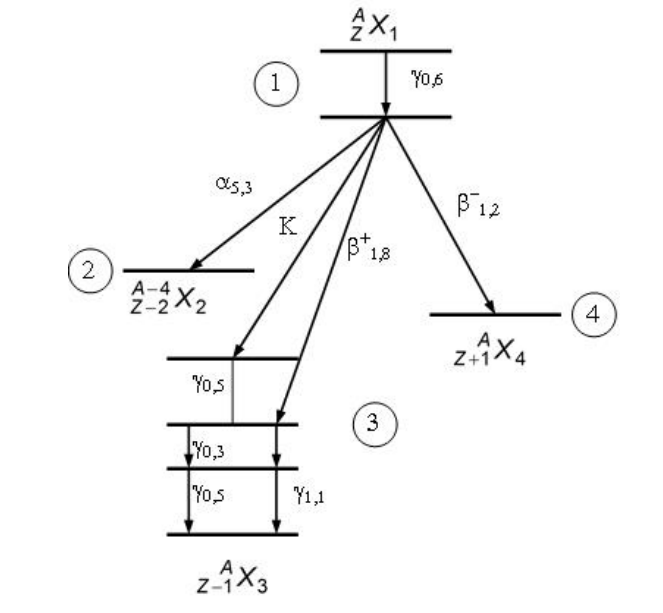
\includegraphics[width=0.45\textwidth]{js5-schema1.png}
\caption{Všeobecná rozpadová schéma}
\label{js5:img:schema1}
\end{figure}

Rádioaktívna $\alpha$ a $\beta$ premena jadier je znázornená šikmou šípkou vľavo či vpravo, spojujúca materské a dcérske jadro v jeho príslušnej energetickej hladine, ktorá sa pri danom procese realizuje. Pri tejto šípke je uvedený typ premeny ($\alpha$, $\beta$, EC\footnote{electron capture - záchyt elektrónu}) a príslušná energia kvanta žiarenia. Deexcitácia vzbudených hladín, t.j. izomérne prechody $\gamma$, sú vyznačené kolmými šípkami spojujúcimi vyššie hladiny s príslušnými výslednými nižšími hladinami, či so základným stavom dcérskeho jadra. Pri šípkach znázorňujúcich jadrové premeny a deexcitácie sa uvádza ich relatívne zastúpenie [$\%$] (pravdepodobnosť, intenzita) - priemerný počet emitovaných kvant (alfa, elektrónov či pozitrónov, fotónov) na 100 premien. V dolnej časti rozpadovej schémy\footnote{pod čiarou dcérskeho jadra, alebo z dôvodu úspory miesta v inom voľnom mieste obrázku} sa uvádza celková energia premeny $Q$ [keV alebo MeV].

Pri vodorovných čiarach, znázorňujúcich základné a excitované energetické stavy jadier, sa v rozpadových schémach uvádzajú ich energie. Hodnoty tejto energie sú vzhľadom k základnému stavu dcérskeho jadra, ktorému sa priradí energia $0$. Základný stav materského jadra má potom energiu $Q$ a prípadné excitované stavy dcérskeho jadra majú príslušné nižšie energie.

\section{Vetvená premena}

Zložitejšia situácia nastáva v prípade vetvenej premeny, kedy sa dané materské jadro premieňa dvomi rôznymi typmi rádioaktivity (s určitou pravdepodobnosťou) na dve rôzne dcérske jadrá s rôznymi energiami základného stavu. Pomer početnosti jednotlivých alternatívnych druhov premien na celkovom počte sa nazýva \textit{vetviaci pomer} (branching ratio). Vetvene sa premieňajúci rádionuklid má v podstate dve premenové konštanty a dva parciálne polčasy rozpadu. Keby sme v myšlienkovom experimente dokázali zablokovať jednotlivé alternatívne typy premeny, dostali by sme pre každú vetvu $1$ a $2$ odlišnú hodnotu rozpadovej konštanty $\lambda_1$, $\lambda_2$ a polčasu rozpadu $T_{1/2,1}$, $T_{1/2,2}$. Celková hodnota rozpadovej konštanty $\lambda_{total}$ potom bude daná súčtom parciálnych hodnôt $\lambda_{total}=\lambda_1+\lambda_2$. Výsledný polčas rozpadu tohto rádionuklidu môžeme považovať za efektívny či celkový polčas oboch vetiev a môžeme ho určiť ako
\begin{equation}
T_{1/2,total}=\dfrac{T_{1/2,1}T_{1/2,2}}{T_{1/2,1}+T_{1/2,2}}
\end{equation} 

Najčastejším typom vetvenej rádioaktívnej premeny je $\beta^-$ + elektrónový záchyt, alebo $\beta^-$ + $\beta^+$. Z prírodných rádioizotopov sa vyskytuje v $^{40}$K, ktorý sa rozpadá $\beta^-$ premenou na $^{40}$Ar ($89\%$) a elektrónovým záchytom na $^{40}$Ca ($11\%$). Vyskytuje sa tiež u niektorých umelých rádionuklidov, napr. $^{152}$Eu, $^{186}$Re, $^{192}$Ir a ďalších.

U niekoľkých rádionuklidov pozorujeme vetvenú premenu $\gamma$ + $\beta$. Býva to vtedy, keď určitý excitovaný stav jadra je metastabilný s dlhým polčasom rozpadu. Vtedy miesto deexcitácie emisiou $\gamma$ fotónu môže s určitou pravdepodbnosťou dochádzať k alternatívnej $\beta$ premene tohoto excitovaného jadra na iné susedné jadro. Extrémnym prípadom je $^{152m}$Eu.

Ďalej je to vetvená premena $\alpha$ + $\beta^-$, vyskytujúca sa pri ťažších jadrách. Pri prírodných rádionuklidoch sa s ňou stretávame v rozpadových radoch uránu a thória, kedy sa izotopy $^{211,212,213}$Bi premieňajú $\alpha$ rozpadom na izotopy tália a $\beta$ rozpadom na izotopy polónia. 

Pri ťažkých rádionuklidoch z oblasti uránov a transuránov sa vyskytujú kombinované premeny $\alpha$ + spontánne štiepenie. Pre urán a ľahšie transurány je podiel spontánneho štiepenia veľmi malý, avšak pre ťažšie transurány býva tento podiel nezanedbateľný, niekedy dokonca rozhodujúci. Napr. $^{252}$Cf sa rozpadá $\alpha$ rozpadom na $^{248}$Cm ($97\%$) a pre zvyšné $3\%$ prípadov sa štiepi na dve ľahšie jadrá z prostriedku periodickej tabuľky a 2-3 neutróny.

\section{Ukážka rozpadových schém}

Na obrázku \ref{js5:img:schema2} sú znázornené niektoré najjednoduchšie typické rozpadové schémy, ktoré si teraz bližšie opíšeme.

\begin{figure}[h!]
\centering
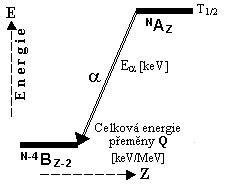
\includegraphics[height=0.3\textwidth]{js5-schema2a.png}
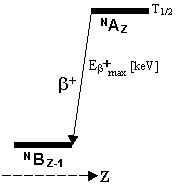
\includegraphics[height=0.3\textwidth]{js5-schema2b.png}
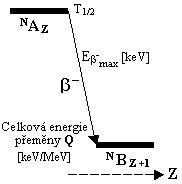
\includegraphics[height=0.3\textwidth]{js5-schema2c.png}
\vspace*{1cm}

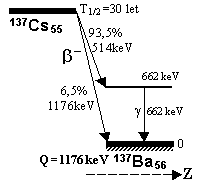
\includegraphics[height=0.3\textwidth]{js5-schema2d.png}
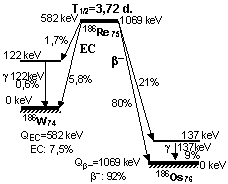
\includegraphics[height=0.3\textwidth]{js5-schema2e.png}
\caption{Najjednoduchšie typické rozpadové schémy}
\label{js5:img:schema2}
\end{figure}

V prvom riadku úplne naľavo je čistý rozpad $\alpha$, kde sa vyžiarením $\alpha$ častice (jadro $^4_2$He) materské jadro $^N_ZA$ premieňa na základný stav dcérskeho jadra $^{N-4}_{Z-2}B$ s nižšou energiou. Jadro $B$ je posunuté doľava o dve miesta, čo odpovedá protónovému číslu $Z-2$, a dole podľa energetického rozdielu. Pri šípke (pre $\alpha$ rozpad sa používa dvojitá šípka) znázorňujúcej vlastnú premenu sa uvádza typ premeny a príslušná energia kvanta emitovaného žiarenia.

Na prostrednom obrázku v prvom riadku je rozpadová schéma čistej rádioaktivity $\beta^+$ ($^N_ZA\rightarrow {^N_{Z-1}B} + e^+ + {\nu}_e$), kde je dcérske jadro $B$ voči materskému jadru $A$ posunuté o jedno miesto doľava, čo odpovedá zníženiu protónového čísla o 1.

Ďalej je rozpadová schéma čistej rádioaktivity $\beta^-$ ($^N_ZA\rightarrow {^N_{Z+1}B} + e^- + \bar{\nu}_e$), kde sa materské jadro $A$ premieňa na základný stav dcérskeho jadra $B$, posunutého o jedno miesto doprava.

Pre jednoduchosť sme zatiaľ odhliadli od skutočnosti, že čistá premena $\alpha$ či $\beta$ na základnú hladinu dcérskeho jadra sa vyskytuje iba v menšom percente prípadov. Väčšinou vzniká dcérske jadro v excitovanom stave s následnou deexcitáciou - kombinovaná rádioaktivita $\alpha +\gamma$ alebo $\beta +\gamma$. V druhom riadku naľavo je znázornená rozpadová schéma $\beta$ rozpadu konkrétneho jadra $^{137}$Cs, ktoré sa s polčasom $T_{1/2}=30$ rokov rozpadá na dcérske jadro $^{137}Ba$, ktoré je stabilné. Na základný stav ide iba asi $6,5\%$ prípadov, zatiaľ čo $93,5\%$ prípadov ide na excitovaný stav jadra $^{137}$Ba s energiou $662\:\unit{keV}$, znázornený vodorovnou čiarou. Zvislou šípkou smerom dole je znázornená deexcitácia tohoto vzbudeného stavuza vyžiarenia fotónu $\gamma$ s energiou $662\:\unit{keV}$.

Na poslednom obrázku (vpravo dole) je ukážka vetvenej rádioaktívnej premeny jedného materského jadra dvomi rôznymi typmi rádioaktivity na dve rôzne dcérske jadrá (konkrétne sa jedná o zjednodušenú schému rádionuklidu $^{186}$Re).

Rozpadové schémy niektorých rádionuklidov sú značne zložité, s radom kaskádových premien a množstvom excitovaných energetických hladín, medzi ktorými nastávajú izomerné prechody doprevádzané kvantami $\gamma$ žiarenia. Tomu odpovedajú aj zložité spektrá takýchto rádionuklidov. Spektrometrická analýza emitovaného žiarenia je potom hlavnou metódou poznávania štruktúry nuklidov.

\section{Rozpadové schémy niektorých rádionuklidov}

\subsection{Trícium $^3$H}

Ak nerátame voľný neutrón, najľahším rádionuklidom je tento izotop vodíku, ktorý sa s polčasom rozpadu 12,3 roku premieňa $\beta^-$ rozpadom na základný stav izotopu hélia $^3$He. Trícium je čistý $\beta$ žiarič s pomerne nízkou maximálnou energiou emitovaných elektrónov $18,6$ keV.

\begin{figure}[h]
\centering
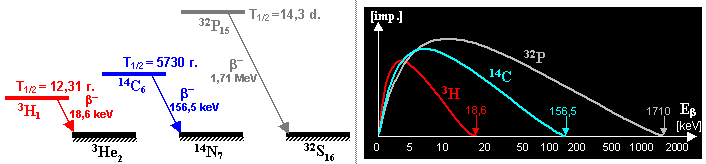
\includegraphics[width=\textwidth]{js5-tritium.png}
\caption{Naľavo rozpadové schémy trícia $^3$H, uhlíku $^{14}$C a fosfóru $^{32}$P. Napravo sú znázornené spojité spektrá $\beta$ rozpadu týchto rádionuklidov s vyznačenou maximálnou energiou žiarenia.}
\label{js5:img:tritium}
\end{figure}

\subsection{Pozitrónové rádionuklidy}

Všetky pozitrónové rádionuklidy, pokiaľ sú obsiahnuté v látkovom prostredí (čo je prakticky vždy), pri anihilácií emitovaných pozitrónov s elektrónmi vysielajú 2 $\gamma$ fotóny s energiou $511$ keV. Gama spektrum \quotedblbase čistých \textquotedblright ~pozitrónových rádionuklidov je tvorené jediným anihilačným píkom $e^+e^-$ $511$ keV s intenzitou blízkou $200\%$ - jedná sa o $^{11}$C, $^{13}$N, $^{15}$O a $^{18}$F. Pri niektorých ťažších pozitrónových rádionuklidoch je zastúpenie pozitrónov nižšie než $100\%$ a tým pádom aj intenzita anihilačného žiarenia je často podstatne nižšia než $200\%$.

\begin{figure}[h]
\centering
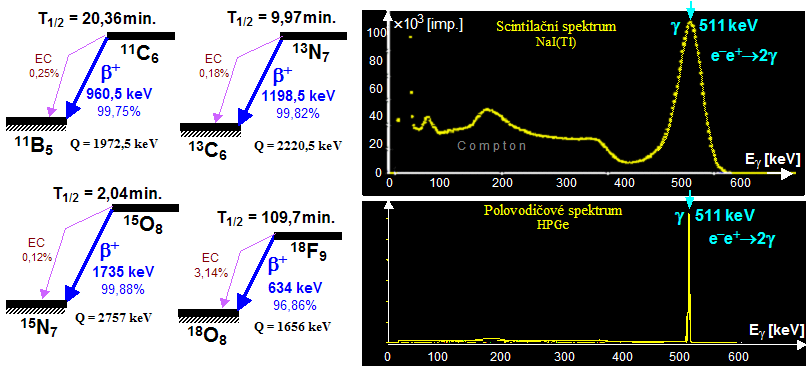
\includegraphics[width=\textwidth]{js5-pozitron.png}
\caption{Naľavo rozpadové schémy rádionuklidov $^{11}$C, $^{13}$N, $^{15}$O a $^{18}$F. Napravo sú znázornené spojité $\gamma$ spektrá ich anihilačného žiarenia.}
\label{js5:img:pozitron}
\end{figure}

\subsection{Technécium}

Pre nukleárnu medicínu je vôbec najdôležitejším rádionuklidom $^{99m}$Tc s polčasom rozpadu $T_{1/2}=6$ hodín, ktoré je čistým žiaričom $\gamma$ s energiou $140$ keV ($88,5\%$). Podrobná rozpadová schéma je v pravej časti obrázku \ref{js5:img:tc99m}. Východzia metastabilná hladina $142$ keV (vzniklá po $\beta$ premene $^{99}$Mo) izomerne prechádza najskôr na hladinu $140,5$ keV, odkiaľ sa vyžaruje základné žiarenie s energiou $140,5$ keV.

\begin{figure}[h]
\centering
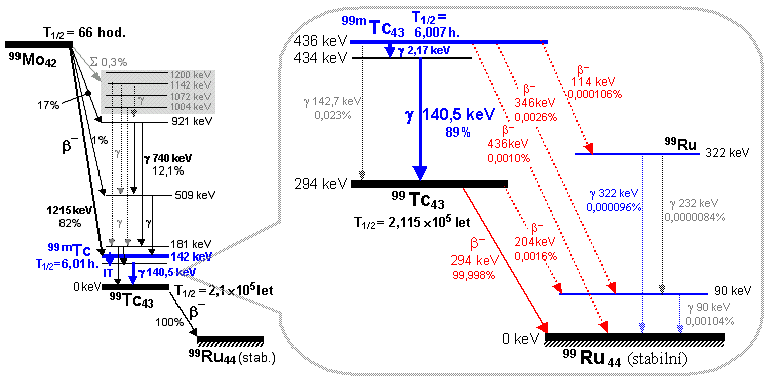
\includegraphics[width=\textwidth]{js5-tc99m.png}
\caption{Podrobná rozpadová schéma $^{99m}$Tc.}
\label{js5:img:tc99m}
\end{figure}

\subsection{Európium}

Európium je ukážkou vetveného rozpadu. S polčasom $13,54$ rokov sa premieňa značne zložitou rozvetvenou rozpadovou schémou. V $28\%$ prípadov dochádza k $\beta^-$ rádioaktivite na excitované hladiny $^{152}$Gd, v $72\%$ prípadov prebieha elektrónový záchyt. 

\begin{figure}[h]
\centering
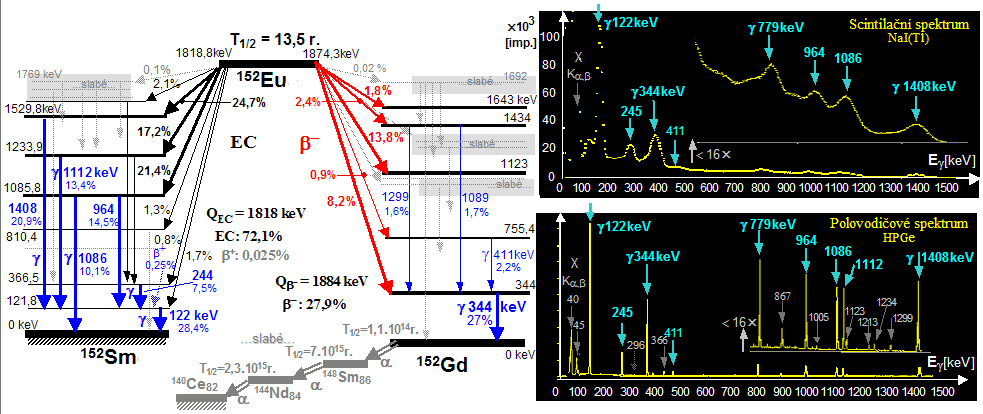
\includegraphics[width=\textwidth]{js5-europium.png}
\caption{Komplikovaná rozpadová schéma $^{152}$Eu.}
\label{js5:img:europium}
\end{figure}

\section{Výberové pravidlá}

Alfa, beta a gama žiarenie môže byť emitované iba v prípade, že sú dodržané zákony zachovania (energie, momentu hybnosti, parity). To vedie k tzv. výberovým pravidlám prechodov. 

Typickým príkladom je \textit{multipolarita gama žiarenia}. Aby sme mohli diskutovať o konkrétnom prípade, je nevyhnutné poznať momenty hybnosti a parity pre každý stav.

\begin{figure}[h]
\centering
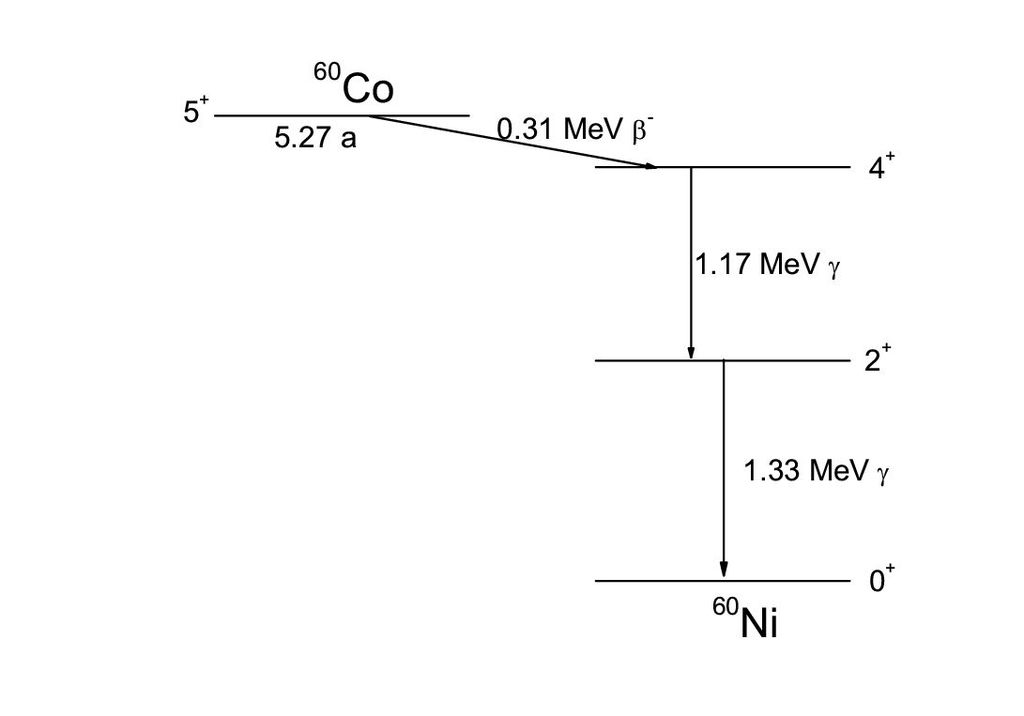
\includegraphics[width=0.5\textwidth]{js5-multipolarita.jpg}
\caption{Rozpadová schéma $^{60}$Co s vyznačenými spinmi a paritou.}
\label{js5:img:multipolarita}
\end{figure}

Multipolarita gama žiarenia môže mať dva druhy: elektrickú a magnetickú multipólovú radiáciu. Dá sa pritom ukázať, že neexistuje monopólové žiarenie ($l=0$). 

Stav jadra je opísaný energiou, momentom hybnosti $J$ (v jednotkách $\hbar$), a paritou, teda správaním sa pri odraze ($+$ alebo $-$). Keďže spin nukleónov je $1/2$ a orbitálny moment hybnosti má celočíselné hodnoty, $J$ môže nadobúdať celo- alebo poločíselné hodnoty.

Elektrické a magnetické multipólové vyžarovanie rovnakého rádu $l$ prenáša rovnaký moment hybnosti $l$, ale rôznu paritu $P$. Platí nasledovné:
\begin{itemize}
\item elektrické multipólové žiarenie: $P=(-1)^l$

Elektrické pole má paritu $P=(-1)^{l+1}$ a magnetické $P=(-1)^{l}$
\item magnetické multipólové žiarenie: $P=(-1)^{l+1}$

Elektrické pole má paritu $P=(-1)^{l}$ a magnetické $P=(-1)^{l+1}$
\end{itemize}



\end{document}